\documentclass[a4paper,11pt,final]{article}
% Pour une impression recto verso, utilisez plutôt ce documentclass :
%\documentclass[a4paper,11pt,twoside,final]{article}

\usepackage[left=2cm,right=2cm,top=2cm,bottom=2cm]{geometry}
\usepackage[english,francais]{babel}
\usepackage[utf8]{inputenc}
\usepackage[T1]{fontenc}
\usepackage[pdftex]{graphicx}
\usepackage{setspace}
\usepackage{hyperref}
\usepackage[french]{varioref}

\newcommand{\reporttitle}{NOM DU JEU}     % Titre
\newcommand{\reportauthor}{Nicolas \textsc{BÉDRINE}} % Auteur
\newcommand{\reportsubject}{Rapport de projet C} % Sujet
\newcommand{\HRule}{\rule{\linewidth}{0.5mm}}
\setlength{\parskip}{1ex} % Espace entre les paragraphes

\hypersetup{
    pdftitle={\reporttitle},%
    pdfauthor={\reportauthor},%
    pdfsubject={\reportsubject},%
}

\begin{document}
  \begin{titlepage}

\begin{center}

\begin{minipage}[t]{0.48\textwidth}
  \begin{flushleft}
	
\includegraphics [width=50mm]{images/logo-telecom.png} \\[0.5cm]
      \textsc{\LARGE Telecom Nancy}
  \end{flushleft}
\end{minipage}
\begin{minipage}[t]{0.48\textwidth}
  \begin{flushright}
    
\includegraphics [width=50mm]{images/logo-ul.jpg} \\[0.5cm]
    \textsc{\LARGE Université de Lorraine}
  \end{flushright}
\end{minipage} \\[1.5cm]


	\textsc{\Large \reportsubject}\\[0.5cm]
	\HRule \\[0.4cm]
	{\huge \bfseries \reporttitle}\\[0.4cm]
	\HRule \\[1.5cm]
	
	\begin{minipage}[t]{0.3\textwidth}
 	 	\begin{flushleft} \large
  		\end{flushleft}
	\end{minipage}
	\begin{minipage}[t]{0.6\textwidth}
  		\begin{flushright} \large
    		\emph{Auteurs :} \\
    		Nicolas \textsc{Bédrine} \\
    		Raphaël \textsc{Moulet} \\
    		Vincent \textsc{Albert} \\
  		\end{flushright}
	\end{minipage}

\vfill

{\large \today{}}

\end{center}

\end{titlepage}

  \cleardoublepage % Dans le cas du recto verso, ajoute une page blanche si besoin
  \renewcommand\thepage{}
  \tableofcontents % Table des matières
  \sloppy          % Justification moins stricte : des mots ne dépasseront pas des paragraphes
  \cleardoublepage
  \renewcommand\thepage{\arabic{page}}
  \setcounter{page}{1}
  
  \section{Présentation du sujet} % Pas de numérotation
\addcontentsline{toc}{section}{Présentation du sujet} % Ajout dans la table des matières

\subsection{Un rapide résumé}
Le jeu que nous nous sommes proposés de réaliser est un beat’em’all et tower defense s’inspirant du jeu BoxHead. Le
principe général est de survivre sur une carte à plusieurs vagues successives d’ennemis. Pour se faire,
le joueur incarne un personnage en vue à la troisième personne qui peut se déplacer, attaquer à distance avec des sorts 
et construire des tours.

\begin{figure}[!ht]
    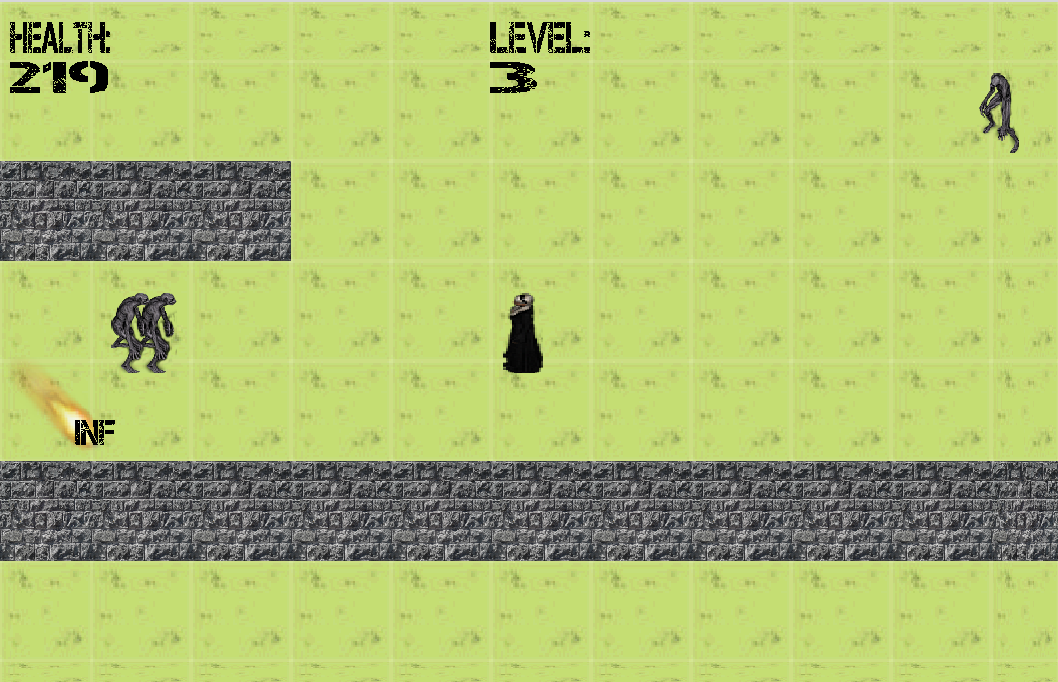
\includegraphics[width=0.5\textwidth]{./images/snapshot1.png}
    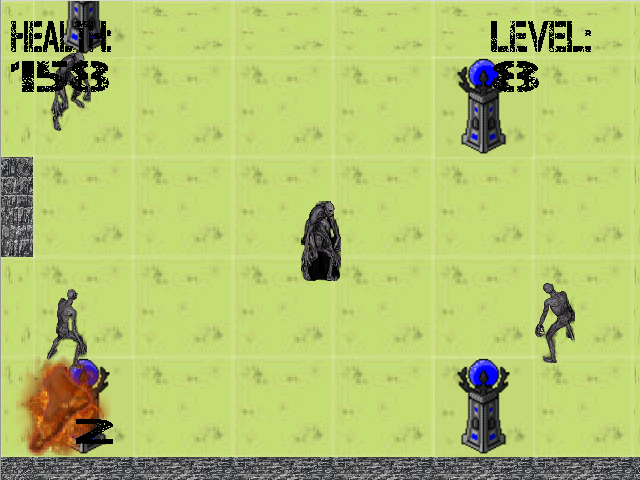
\includegraphics[width=0.5\textwidth]{./images/snapshot2.png}
    \caption{Snapshots}
\end{figure}

\subsection{Une licence pour les protéger tous}

Le logiciel et l'ensemble des sources sont sous licence CC BY-NC-SA 3.0 FR. \\
Le partage et l'adaptation du logiciel sont permises à condition de ne pas l'utiliser
commercialement, d'indiquer les changements effectués, de référencer l’œuvre originale et 
de conserver la même licence lors d'une diffusion ultérieure.

\subsection{Le cahier des charges}

Afin de gérer au mieux le projet, nous nous proposons d’établir un cahier des charges minimal dont les
caractéristiques se retrouveront dans toute version finale du projet. En plus de cela, nous établirons une liste
non ordonnée de fonctionnalités qu’il semble de prime abord intéressant d’implémenter. Leur mise en place
découlera de leur difficulté ainsi que du temps disponible. \\
Cahier des charges minimal :
\begin{itemize}
\item Lancement d’une partie sur une carte unique
\item Interaction avec le clavier pour se déplacer et attaquer
\item Gestion de l’interaction avec l’environnement (collision, ...)
\item Création d’un dispositif de défense
\item Menu d’accueil
\end{itemize}
Fonctionnalités optionnelles :
\begin{itemize}
\item Capacités spéciales à usage limité
\item Difficulté croissante des ennemis dans le temps (ennemis plus rapides, plus résistants, ...)
\item Mode coopératif/deathmatch à deux en réseau ou sur le même clavier
\item Mini mode aventure
\item Menu pause
\item Choix de la difficulté générale
\item Éditeur de cartes et choix de carte
\end{itemize}
  \cleardoublepage
  \section{Organisation}

\subsection{Les outils utilisés}

Le projet a été codé en langage C sous systèmes de type Unix. L’affichage graphique a été réalisé à l’aide de la
bibliothèque SDL qui est déjà utilisée dans de nombreux jeux. Les sprites sont libres de droits. Étant donné l’ampleur du projet et le
nombre de participants, nous nous sommes convenus d’utiliser le gestionnaire de version git. Un dépôt public a été créé sur Github et est accessible à l'adresse suivante : \url{https://github.com/Neressea/projetC}

\subsection{Le planning initial}

Afin d'achever au mieux les objectifs que nous nous étions fixés, nous avons dressé un planning optimal des tâches à effectuer.

\subsection{Le schéma des fichiers et des fonctionnalités}


\begin{figure}[!ht]
    \center
    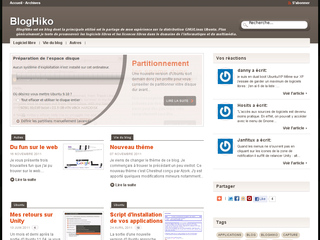
\includegraphics[width=0.5\textwidth]{./images/bloghiko.jpg}
    \caption{BlogHiko | 50\% de la largeur de la page}
\end{figure}



  \cleardoublepage
  \section{La phase de développement}

\subsection{Les attentes atteintes}

L'ensemble du cahier des charges minimal a été implémenté. De plus, la difficulté est proportionnelle au niveau du joueur. En effet, le nombre d'ennemis dépend du niveau du joueur, et donc des ennemis qu'il a déjà vaincu. Nous avons aussi ajouté une attaque à usage limitée. Des items sont laissés par les ennemis vaincus pour régénérer les points de vie du héros ou son sort limité. Enfin, la vue a été adaptée pour que la carte est redimensionnable en cours de partie. 

\subsection{Ce qui reste inachevé}

Malheureusement, nous n'avons pas réussi à mettre en pratique nos autres idées. Cependant, nous avons tout de même préparé l'implémentation d'autres fonctionnalités. Ainsi, même si l'éditeur de cartes n'a pas été réalisé, le code a été adapté afin de pouvoir charger des fichiers textes formatés pour faciliter son ajout par la suite. 

De la même manière, bien que la vue soit prête pour la modification des touches, et qu'il existe une fonction permettant de modifier les contrôles utilisateurs, nous n'avons pas eu le temps de lier les deux.

\subsection{Les problèmes rencontrés}

	\subsubsection{Quelques problèmes de communication}
 
En nous confrontant pour la première fois à un travail de groupe de cette ampleur, nous avons rencontré quelques difficultés, dont certaines communicationnelles. En effet, lors de la recherche de sprites, nous avons commencé par les boules de feu ; puis nous nous sommes concertés pour la recherche des boules de glace. Cependant à cause d'un quiproquo, nous avons temporairement fini avec des sprites de cornets de glace. 

	\subsubsection{De la mémoire et des fuites}

Après plusieurs longues séances de codage consécutives

	\subsubsection{Gestion événementielle}
	
	Nous n'arrivions pas dans un premier temps à gérer l'appuie de plusieurs touches en même temps. Nous avons alors changer notre Wait\_Event par un Poll\_Event. Ce dernier a comme avantage de garder en mémoire plusieurs évènements, contrairement à Wait\_Event qui les gèrent un par un. Les évènements étant stockés dès le premier appel de la fonction Poll\_Event, un switch(Poll\_Event) n'est pas nécessaire. Nous avons ensuite décidé de créer un tableau de booléen contenant les états de chaque touche nécessaire au jeu. Il a donc fallu contrôler à la fois lorsqu'une touche est pressée, mais aussi lorsqu'elle ne l'est plus. Ce tableau nous a permis de gérer les évènements de manière plus lisible, mais aussi de gérer grâce à un if l'état de plusieurs touches à la fois, permettant de gérer l'appuie de plusieurs touches. 

	\subsubsection{La vue et le modèle}
Collisions et vue déplaçable.

  \cleardoublepage
  
  \setcounter{page}{0}
  \thispagestyle{empty}
  \section*{Références et autres sources d'inspiration}
\addcontentsline{toc}{section}{Références}

\url{http://blog.hikoweb.net/index.php?post/2011/11/06/Exemple-de-rapport-en-LaTeX} \\
\emph{Source pour le template \LaTeX ayant servi à la rédaction de ce rapport.} \\

\url{http://www.crazymonkeygames.com/Boxhead-2Play-Rooms.html} \\
\emph{Source d'inspiration du jeu.} \\

\url{https://wiki.libsdl.org/} \\
\emph{Wiki de la SDL 2.0.} \\

\url{http://gnurou.org/} \\
\emph{Nous nous sommes inspirés des algorithmes de ce site pour la gestion des événements.} \\

\url{http://jeux.developpez.com/tutoriels/sdl-2/guide-migration/} \\
\emph{Guide de migration de passage de la SDL 1.2 à la SDL 2.0. Ce site nous a été utile étant donné
que nous avions déjà programmé avec la SDL 1.2 auparavant.} \\

\url{https://creativecommons.org/licenses/by-nc-sa/3.0/fr/} \\
\emph{Licence s'appliquant au logiciel.} \\

\url{http://www.pioneervalleygames.com/free-resources.html} \\
\url{http://opengameart.org/} \\
\emph{Sources des sprites libres utilisées dans le jeu.} \\

\url{https://www.draw.io/} \\
\emph{Site qui a servi à la création de l'UML}

\url{https://app.smartsheet.com}
\emph{Site qui a servi à la création du Gantt}

\url{http://soundbible.com/} \\
\url{http://www.audiomicro.com/} \\
\url{http://incompetech.com/music/royalty-free/} \\
\emph{Sources des fichiers audio utilisés dans le jeu.} \\

%% SPRITES %%

\end{document}

